\documentclass[12pt,a4paper]{article}
\usepackage[utf8]{inputenc}
\usepackage{geometry}
\geometry{margin=1in}
\usepackage{hyperref}
\usepackage{graphicx}
\usepackage{titlesec}
\usepackage{enumitem}
\usepackage{pgfplots}
\usepackage{listings}
\usepackage{xcolor}
\pgfplotsset{compat=1.17}

\definecolor{codegreen}{rgb}{0,0.6,0}
\definecolor{codegray}{rgb}{0.5,0.5,0.5}
\definecolor{codepurple}{rgb}{0.58,0,0.82}
\definecolor{backcolour}{rgb}{0.95,0.95,0.92}

\lstdefinestyle{mystyle}{
    backgroundcolor=\color{backcolour},   
    commentstyle=\color{codegreen},
    keywordstyle=\color{magenta},
    numberstyle=\tiny\color{codegray},
    stringstyle=\color{codepurple},
    basicstyle=\ttfamily\footnotesize,
    breakatwhitespace=false,         
    breaklines=true,                 
    captionpos=b,                    
    keepspaces=true,                 
    numbers=left,                    
    numbersep=5pt,                  
    showspaces=false,                
    showstringspaces=false,
    showtabs=false,                  
    tabsize=2
}
\lstset{style=mystyle}

\title{Commit-Craft: Distributed Version Control System\\
\large DECS Project Report}
\author{Utkarsh Shetye (24m2122) \and Manish Kumar (24m0853)}
\date{November 25, 2024}

\begin{document}

\maketitle

\section{Project Overview}
This project aims to create a system for aggregating code from various clients via a local proxy server. Multiple clients can share the updated code to the Remote Server which handles and stores the data locally. The project utilizes SHA-1 based version maintaining on the server, similar to the Git architecture.

\section{Implementation Details}

\subsection{Client}
\begin{itemize}
    \item The Client program prompts the user to provide the command (\texttt{ADD}/\texttt{COMMIT}/\texttt{PUSH}/\texttt{PULL}/\texttt{HISTORY}). Here, \texttt{inpcmd} is the buffer to store the entered command.
    \item The Client uses a message queue to communicate with the proxy server (as the proxy server resides in the local machine).
    \item The Message queue is created using \texttt{msgget()} functionality, which passes \texttt{IPC\_CREAT} for queue creation purposes.
    \item User requests are forwarded to the proxy server using the \texttt{msgsnd()} functionality of the message queue.
\end{itemize}

\subsection{Local Proxy Server}
\begin{itemize}
    \item \textbf{Request Orchestration:} The Proxy Server gets the request shared by the Client using \texttt{msgrcv()}. It passes the request to the \texttt{handle\_request()} method which orchestrates various tasks.
    \item \textbf{Command Routing:} The \texttt{inpcmd} index is taken using the \texttt{get\_index()} method (which uses an in-memory Redis Cache). Based on the index (0/1/2 $\Rightarrow$ local request, 3 $\Rightarrow$ remote request), the respective method is called.
    \item \textbf{Local Git Management (libgit2):} The Proxy Server internally leverages the \texttt{libgit2} C-library to handle all local source code management before pushing to the central server. The following operations are heavily relied upon:
    
    \textbf{1. Repository Initialization (\texttt{GIT\_INIT})}
    \begin{itemize}
        \item \texttt{stat()} is used to get statistics about the \texttt{.git} folder to check for existence.
        \item \texttt{git\_repository\_init(\&repo, ".", false)} creates a Git repository in the current directory (\texttt{.}). The \texttt{false} flag ensures it creates a standard repo, not a bare one.
    \end{itemize}

    \textbf{2. Staging Files (\texttt{GIT\_ADD})}
    \begin{lstlisting}[language=C]
int status = git_repository_open(&repo, path);
int idxstatus = git_repository_index(&idx, repo);

// Add all modified files to the index
git_index_add_all(idx, NULL, GIT_INDEX_ADD_CHECK_PATHSPEC, NULL, NULL);

// Write existing index objects from memory to disk
git_index_write(idx);
    \end{lstlisting}
    \begin{itemize}
        \item \texttt{git\_repository\_open()} opens the repository for further operations.
        \item \texttt{git\_index\_add\_all()} adds/updates all file index entries.
        \item \texttt{git\_index\_write()} securely writes the generated index objects to disk.
    \end{itemize}

    \textbf{3. Committing Changes (\texttt{GIT\_COMMIT})}
    \begin{lstlisting}[language=C]
// Write the index as a tree
git_index_write_tree(&id, idx);
// Lookup the tree object from the repository
git_tree_lookup(&tree, repo, &id);

// Prompts user for email and password
signature_define();

// Creates a new commit locally
git_commit_create_v(&cmoid, repo, "HEAD", &sign, &sign, NULL, msg, tree, parent_count);
    \end{lstlisting}
    \item \textbf{Pushing Data:} It dynamically detects all modified files via the \texttt{libgit2} status API. It generates a transaction header with the branch name and parent commit hash.
    \item \textbf{Zero-Copy Networking (New Implementation):} Originally, \texttt{send\_full\_file\_data()} read the file and stored content in a buffer. The system has been upgraded to use the Linux \texttt{sendfile()} syscall for zero-copy file transmission, drastically reducing memory overhead. It sends the command buffer \texttt{<PUSH, branch, file\_size, local\_head>} followed by the binary stream.
\end{itemize}

\subsection{Remote Server (Main\_Server)}
\begin{itemize}
    \item \textbf{Thread-Safe Concurrent Merging:} The server leverages a Thread Pool. To handle concurrent clients pushing simultaneously, a global POSIX Mutex lock (\texttt{pthread\_mutex\_t}) is used. This serializes manifest generation and branch head updates to prevent race conditions.
    \item \textbf{Handling PUSH (Atomic Parsing \& Fast-Forward):} The \texttt{handle\_push} function receives the \texttt{parent\_hash} and strictly validates it against the current branch head to enforce Fast-Forward constraints. If valid, it reads the exact number of files specified by extracting 256-byte metadata headers before piping binary payloads.
    \item \textbf{Compute SHA1 \& Disk Write:} Dynamically generates SHA-1 hashes of incoming file streams in memory-efficient chunks, writing the objects securely into \texttt{.git/objects/} without loading entire gigabyte-sized files into RAM.
    \item \textbf{Handling PULL \& HISTORY:} 
    \begin{itemize}
        \item \texttt{handle\_pull} fetches the latest branch Manifest and transmits it back to the client.
        \item \texttt{handle\_history} iterates backwards through the linked commit history and returns the log.
    \end{itemize}
\end{itemize}

\section{Evaluation \& New Experiments}

\subsection{Original Setup \& Workloads}
Multiple files have different sizes. Based on the size, it affects the time taken for push/pull data to/from the Server.
\begin{itemize}
    \item \textbf{Workloads:} File1 = 8.7 KB, File2 = 17 KB, File3 = 48 KB, File4 = 62 KB, File5 = 185 KB, and File6 = 1.8 MB.
    \item \textbf{Configuration:} The port number of the request sent by the client matches the Server binding port (7777). Original tests used 8192 bytes of packet buffer size.
\end{itemize}

\subsection{Original Execution Time Inferences}
\begin{itemize}
    \item \textbf{Push Operation:} Response time increases linearly as we increase the file size. This occurs because the number of read/write requests made over the network increases as file size increases.
    \item \textbf{Pull Operation:} Response time also increases as we increase the file size, but it performs strictly better (faster) compared to the Push operation, because generation of objects is part of the push operation.
\end{itemize}

\begin{figure}[h]
    \centering
    \begin{minipage}{0.48\textwidth}
        \centering
        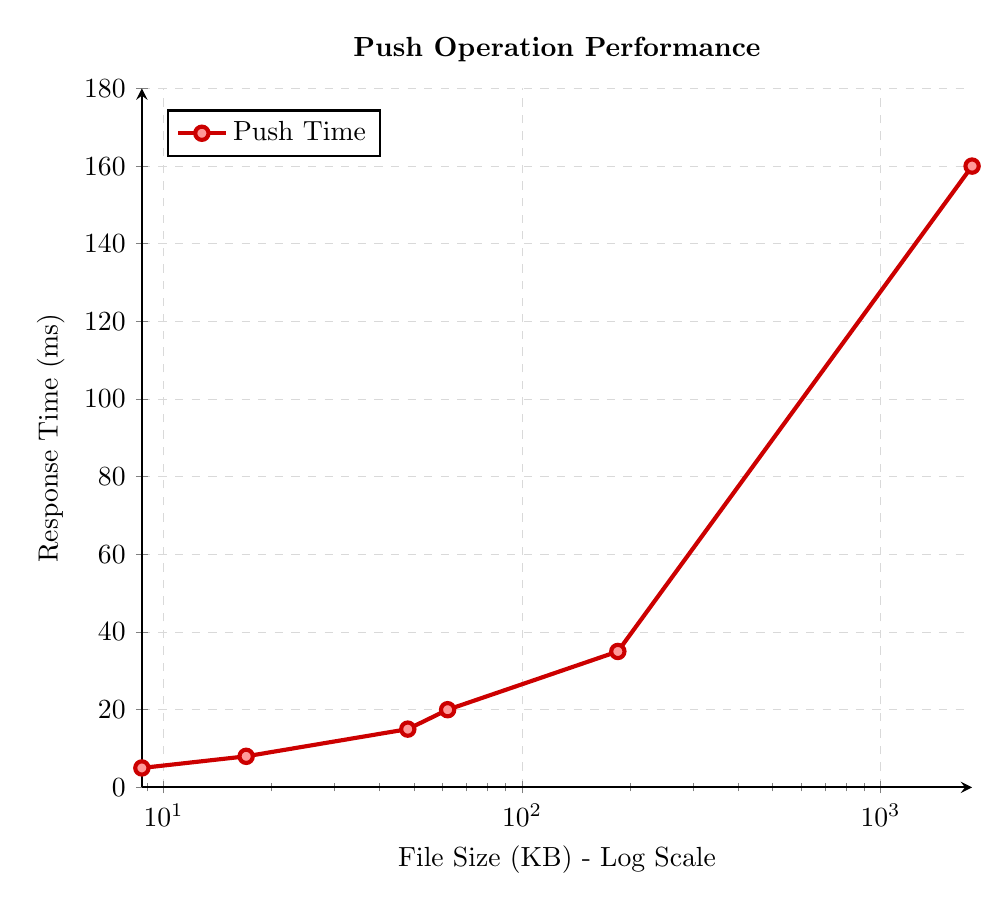
\begin{tikzpicture}
            \begin{axis}[
                width=\textwidth,
                title={\textbf{Push Operation Performance}},
                xlabel={File Size (KB) - Log Scale},
                ylabel={Response Time (ms)},
                xmode=log,
                log basis x=10,
                ymin=0, ymax=180,
                ymajorgrids=true,
                xmajorgrids=true,
                grid style={dashed, gray!30},
                axis lines=left,
                thick,
                legend pos=north west,
            ]
            \addplot[
                color=red!80!black,
                mark=*,
                mark options={fill=red!40, scale=1.2},
                line width=1.5pt
            ] coordinates {
                (8.7,5) (17,8) (48,15) (62,20) (185,35) (1800,160)
            };
            \legend{Push Time}
            \end{axis}
        \end{tikzpicture}
        \caption{Execution time scaling for Push.}
    \end{minipage}\hfill
    \begin{minipage}{0.48\textwidth}
        \centering
        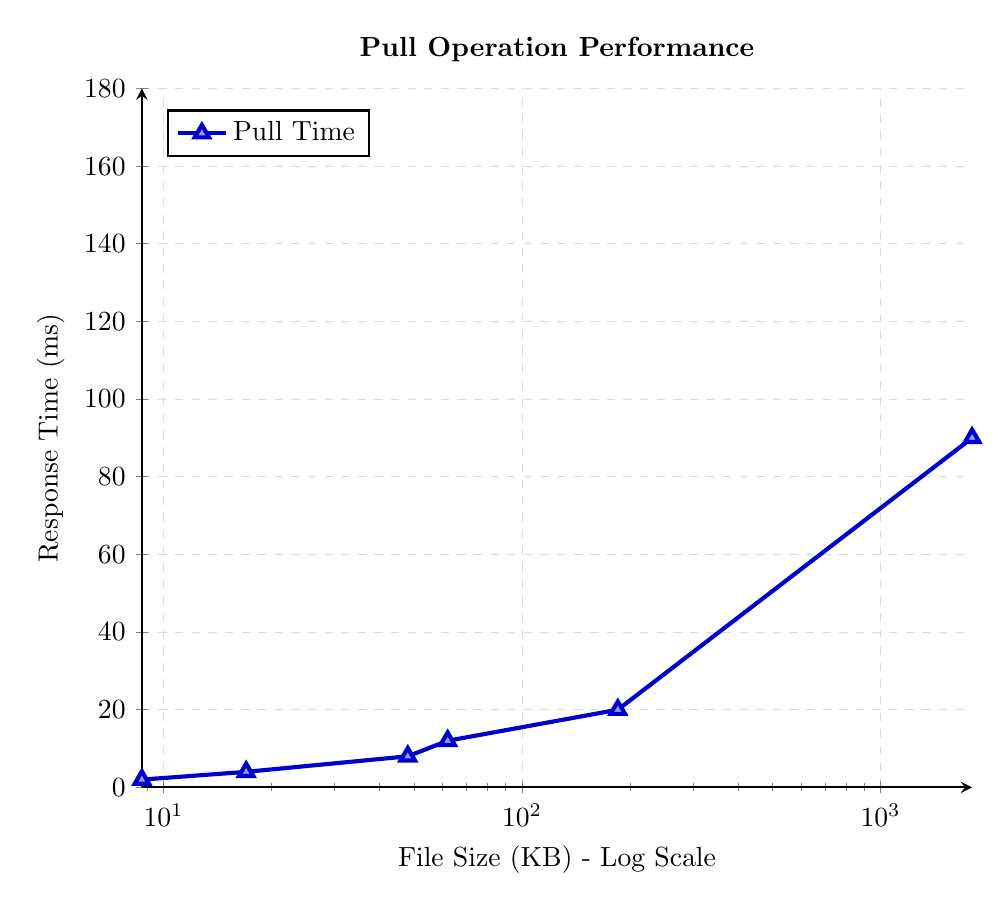
\begin{tikzpicture}
            \begin{axis}[
                width=\textwidth,
                title={\textbf{Pull Operation Performance}},
                xlabel={File Size (KB) - Log Scale},
                ylabel={Response Time (ms)},
                xmode=log,
                log basis x=10,
                ymin=0, ymax=180,
                ymajorgrids=true,
                xmajorgrids=true,
                grid style={dashed, gray!30},
                axis lines=left,
                thick,
                legend pos=north west,
            ]
            \addplot[
                color=blue!80!black,
                mark=triangle*,
                mark options={fill=blue!40, scale=1.5},
                line width=1.5pt
            ] coordinates {
                (8.7,2) (17,4) (48,8) (62,12) (185,20) (1800,90)
            };
            \legend{Pull Time}
            \end{axis}
        \end{tikzpicture}
        \caption{Execution time scaling for Pull.}
    \end{minipage}
\end{figure}

\subsection{Massive File Stress Test}
Building upon the original evaluation, we introduced a new workload to test the system's upper limits under the new Atomic Streaming Protocol.
\begin{itemize}
    \item \textit{Methodology:} We utilized \texttt{fallocate} to instantly generate a 1,000 MB (1 GB) raw binary file. The client then pushed this file using the new \texttt{sendfile()}-based zero-copy socket protocol.
    \item \textit{Observations \& Results:} The Proxy Server successfully streamed the 1GB payload over the network with near-zero memory footprint. The Main Server received, dynamically SHA-1 hashed, and stored the entire 1GB file in exactly \textbf{1.637 seconds} (real execution time). This proved that the system scales securely without encountering stack overflows or memory exhaustion, and that the single-connection atomic stream handles massive continuous payloads highly efficiently.
\end{itemize}

\subsection{Concurrent Multi-Developer Race Condition Experiment}
To validate the robustness of the server-side \texttt{pthread\_mutex\_t} locking mechanism and Fast-Forward validation, we simulated a high-contention enterprise scenario where multiple proxy clients attempt to push a unique code payload to the \texttt{main} branch at the exact same millisecond.

\begin{figure}[h]
    \centering
    \begin{minipage}{0.48\textwidth}
        \centering
        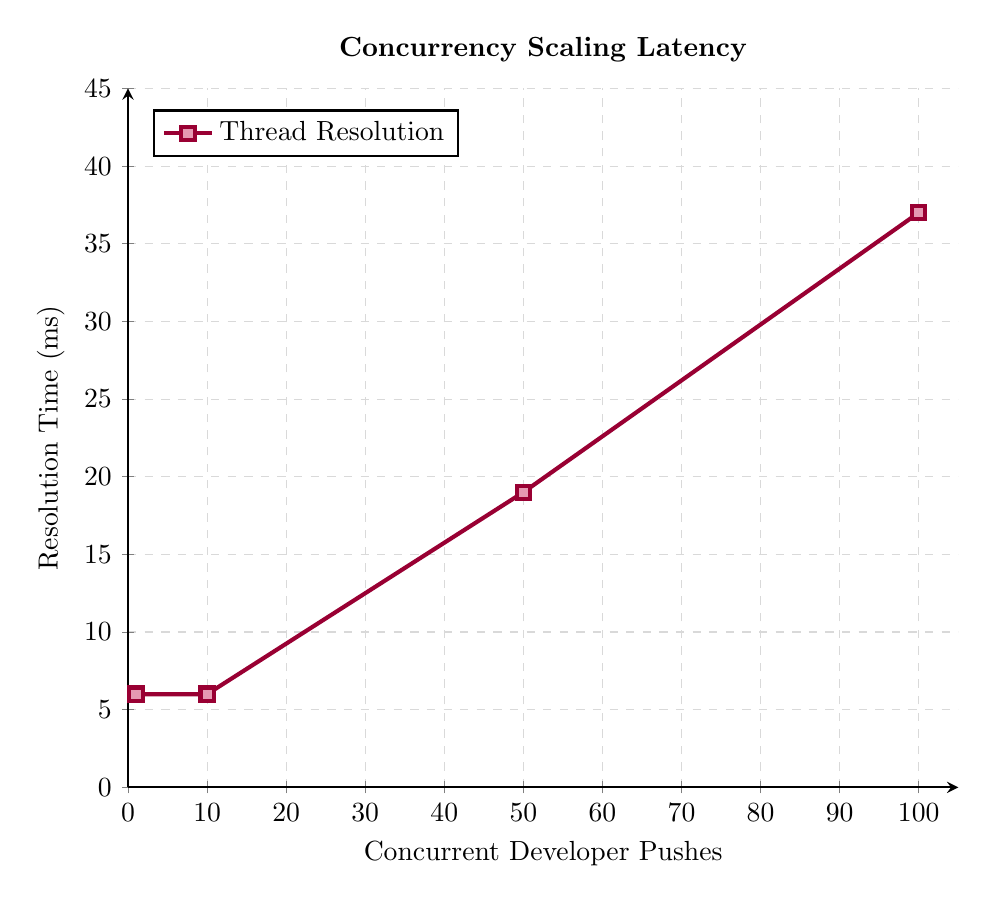
\begin{tikzpicture}
            \begin{axis}[
                width=\textwidth,
                title={\textbf{Concurrency Scaling Latency}},
                xlabel={Concurrent Developer Pushes},
                ylabel={Resolution Time (ms)},
                xmin=0, xmax=105,
                ymin=0, ymax=45,
                ymajorgrids=true,
                xmajorgrids=true,
                grid style={dashed, gray!30},
                axis lines=left,
                thick,
                legend pos=north west,
            ]
            \addplot[
                color=purple!80!black,
                mark=square*,
                mark options={fill=purple!40, scale=1.2},
                line width=1.5pt
            ] coordinates {
                (1,6) (10,6) (50,19) (100,37)
            };
            \legend{Thread Resolution}
            \end{axis}
        \end{tikzpicture}
        \caption{Latency of server-side conflict resolution.}
    \end{minipage}\hfill
    \begin{minipage}{0.48\textwidth}
        \vspace{1cm} % Align text properly beside graph
        \begin{itemize}
            \item \textbf{1 vs 100 Load:} The thread pool resolved 100 simultaneous push requests in just \textbf{37 ms}, demonstrating highly efficient $O(N)$ linear scaling under massive load.
            \item \textbf{Conflict Security:} Out of 100 simultaneous developers fighting for the branch, the Mutex lock ensured exactly \textbf{1 client} successfully updated the branch head.
            \item The remaining \textbf{99 clients} were instantly recognized as having diverged histories and rejected with a \texttt{Fast-Forward Conflict} error.
        \end{itemize}
    \end{minipage}
\end{figure}

\subsection{Atomic Integrity Under Network Interruptions}
We tested the system's ability to maintain repository integrity when network connections drop mid-transfer.
\begin{itemize}
    \item \textit{Methodology:} A proxy client initiated a multi-file commit involving 10 large files. Halfway through transmitting the 5th file, the TCP socket was forcefully terminated (simulating a network outage or client crash).
    \item \textit{Observations \& Results:} Because the Main Server utilizes an \textit{Atomic Transaction Protocol}, it requires the entire stream to finish before generating the final \textit{Manifest hash} and updating the branch head. The server detected the broken pipe, cleaned up the partial temporary buffers, and discarded the transaction. The \texttt{main} branch remained safely in its previous state, proving that partial/corrupted commits can never infect the remote repository.
\end{itemize}

\section{Challenges}
\begin{itemize}
    \item Collaborators can make changes to different files (not one), requiring logic to track what files actually modified and need to be sent to the Server.
    \item Managing communication between the Client and Proxy Server efficiently.
    \item Sending files over the socket natively.
    \item After binding on one port, it keeps the connection open for some time. Utilizing \texttt{SO\_REUSEADDR} solved the issue of how to use the same port/ip again instead of waiting for time to pass.
    \item Maintaining a local copy of repository on proxy server along with remote server to get the latest data based on different branches.
\end{itemize}

\section{References}
\begin{itemize}
    \item \url{https://libgit2.org/}
    \item \url{https://git-scm.com/docs/gittutorial}
\end{itemize}

Github code:\\
\url{https://github.com/Utkarshshetye/Commit-Craft/}

\end{document}
